\documentclass[a4paper,12pt]{article} 


\usepackage[T2A]{fontenc}			
\usepackage[utf8]{inputenc}			
\usepackage[english,russian]{babel}	

\usepackage{graphicx, scalerel}    
\usepackage{wrapfig}               
\usepackage[14pt]{extsizes}        
\usepackage[warn]{mathtext}       
\usepackage{indentfirst}      
\usepackage[margin = 25mm]{geometry}
\usepackage[table,xcdraw]{xcolor} 
\usepackage{amsmath,amsfonts,amssymb,amsthm,mathtools}
\usepackage{wasysym}                
\usepackage{upgreek}                
\usepackage{caption}
\usepackage{multirow}
\captionsetup{labelsep=period}
\usepackage[font=small,labelfont=bf]{caption}
\usepackage{gensymb}
\usepackage[unicode, pdftex]{hyperref}
\usepackage{tikz}
\usetikzlibrary{positioning}
\usepackage{fancyhdr}
\pagestyle{fancy}
\setlength\fboxsep{3pt} % Отступ рамки \fbox{} от рисунка
\setlength\fboxrule{1pt} % Толщина линий рамки \fbox{}
\newcommand{\tocsection}[1]{\section*{#1} \addcontentsline{toc}{section}{#1}}
\newcommand{\tocsubsection}[1]{\subsection*{#1} \addcontentsline{toc}{subsection}{#1}}
\renewcommand{\cftsecleader}{\cftdotfill{\cftdotsep}}

\def\fillandplacepagenumber{%
	\par\pagestyle{empty}%
	\vbox to 0pt{\vss}\vfill
	\vbox to 0pt{\baselineskip0pt
		\hbox to\linewidth{\hss}%
		\baselineskip\footskip
		\hbox to\linewidth{%
			\hfil\thepage\hfil}\vss}}

\begin{document}
		\newcommand{\HRule}{\rule{\linewidth}{0.7mm}} % Defines a new command for the horizontal lines, change thickness here

\begin{center}
	\large\textbf{Московский Физико-Технический Институт}\\
	\large\textbf{(государственный университет)}
	
	\vfill
	

	
	\Large Вычислительная математика
	%----------------------------------------------------------------------------------------
	%	TITLE SECTION
	%----------------------------------------------------------------------------------------
	
	\HRule
	\\[0.4cm]
	{ \huge \bfseries Лабораторная работа №9}
	\\[0.4cm] % Title of your document
	\HRule
	\\[0.5cm]
	
	\ \\
	\textbf{\large Автор:} \\	
	\large Овсянников Михаил Б01-008\\
	\vfill
	\hspace*{-0.8 cm}
\includegraphics[width=100 pt]{./Include/frkt_logo.pdf}\\
	\large Долгопрудный, 2023
\end{center}

\thispagestyle{empty}

\newpage
\setcounter{page}{2}
\fancyfoot[c]{\thepage}
\fancyhead[L] {Лабораторная работа №9}
\fancyhead[R]{}

		\tableofcontents
		\newpage
		
		\tocsection{Цель}
	 	Найти собственные значения и собственные функции заданного уравнения.
			
		\tocsection{Теоретические сведения}
		\tocsubsection{Общая задача}

		Задача нахождения собственных значений и функций дифференциального уравнения называется задачей Штурма-Лиувилля.
		Выглядит это так:
		\begin{equation*}
			\begin{cases}
			\frac{d}{dx}\left[k(x)\frac{dy}{dx}\right] + \left[p(x) + \lambda q(x)\right]y = 0, \\
			\mu_0 y(0) + \mu_1 y'(0) = 0, \\
			\nu_0 y(x_L) + \nu_1 y'(x_L) = 0.
			\end{cases}
		\end{equation*}
	
		Здесь $\lambda$ -- искомое собственное значение.
	
		Такую задачу решают с помощью метода стрельбы, используя $\lambda$ как параметр. Останавливаться на данном методе не будем, поскольку он был описан в лабораторной работе №8, а перейдем сразу к уже данной задаче.
	
		\tocsection{Сама система}
		\tocsubsection{Постановка задачи}
		В качестве примера задачи на поиск собственных значений и функций был выбран номер \textbf{XI.9.19} второй части сборника Аристовой и Лобанова.
		
		По теории речеобразования речевой аппарат человека представляет собой единую акустическую систему, возбуждаемую периодическими колебаниями голосовых связок либо турбулентным шумом. При этом голосовой тракт можно рассматривать как резонатор или фильтр, собственные частоты и собственные функции которого определятся из решения следующей спектральной задачи:
		\begin{equation*}
			\begin{cases}
				(S(x)\Psi'_x(x))'_x + \lambda^2 S(x)\Psi(x) = 0, \;\;\;\;\; 0 < x < L, \\
				\Psi'_x(0) = 0, \\
				8\sqrt{S(L)}\Psi'_x(L) + 3\pi\sqrt{\pi}\Psi(L) = 0.
			\end{cases}
		\end{equation*}
		
		Здесь $x$ -- расстояние вдоль оси распространения волн от голосовых связок до рассматриваемого сечения голосового тракта (рис. \ref{VOICE}). Функция $S(x)$ -- функция площади сечения голосового тракта вдоль оси распространения волн; $L$ -- длина голосового тракта.
		
		\begin{figure}[h!]
			\centering
			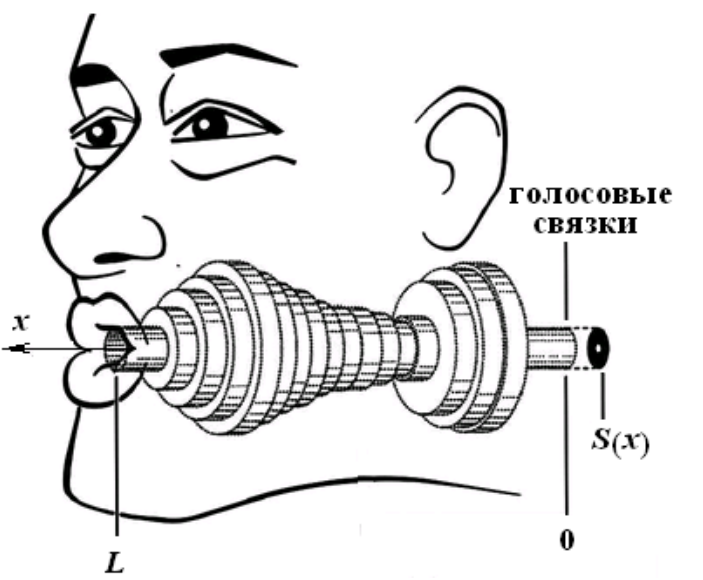
\includegraphics[width=0.9\linewidth]{Pictures/Voice.png}
			\caption{Аппроксимация голосового тракта}
			\label{VOICE}
		\end{figure}
		
		\newpage
		Функция $S(x)$ задана таблично:
		\begin{table}[h!]
			\centering
			\begin{tabular}{|c|c|ccc|c|c|ccccc}
				\cline{1-2} \cline{6-7} \cline{11-12}
				$x$, мм & $S(x)$, мм$^2$ &  &  &  & $x$, мм & $S(x)$, мм$^2$ &  &  & \multicolumn{1}{c|}{} & \multicolumn{1}{c|}{$x$, мм} & \multicolumn{1}{c|}{$S(x)$, мм$^2$} \\ \cline{1-2} \cline{6-7} \cline{11-12} 
				0,0     & 78,2           &  &  &  & 57,5    & 515,9          &  &  & \multicolumn{1}{c|}{} & \multicolumn{1}{c|}{115,0}   & \multicolumn{1}{c|}{7,8}            \\ \cline{1-2} \cline{6-7} \cline{11-12} 
				2,5     & 66,4           &  &  &  & 60,0    & 486,6          &  &  & \multicolumn{1}{c|}{} & \multicolumn{1}{c|}{117,5}   & \multicolumn{1}{c|}{13,7}           \\ \cline{1-2} \cline{6-7} \cline{11-12} 
				5,0     & 43,0           &  &  &  & 62,5    & 453,3          &  &  & \multicolumn{1}{c|}{} & \multicolumn{1}{c|}{120,0}   & \multicolumn{1}{c|}{23,4}           \\ \cline{1-2} \cline{6-7} \cline{11-12} 
				7,5     & 39,1           &  &  &  & 65,0    & 434,8          &  &  & \multicolumn{1}{c|}{} & \multicolumn{1}{c|}{122,5}   & \multicolumn{1}{c|}{27,4}           \\ \cline{1-2} \cline{6-7} \cline{11-12} 
				10,0    & 33,2           &  &  &  & 67,5    & 420,0          &  &  & \multicolumn{1}{c|}{} & \multicolumn{1}{c|}{125,0}   & \multicolumn{1}{c|}{23,4}           \\ \cline{1-2} \cline{6-7} \cline{11-12} 
				12,5    & 25,4           &  &  &  & 70,0    & 420,7          &  &  & \multicolumn{1}{c|}{} & \multicolumn{1}{c|}{127,5}   & \multicolumn{1}{c|}{21,2}           \\ \cline{1-2} \cline{6-7} \cline{11-12} 
				15,0    & 31,3           &  &  &  & 72,5    & 437,2          &  &  & \multicolumn{1}{c|}{} & \multicolumn{1}{c|}{130,0}   & \multicolumn{1}{c|}{18,5}           \\ \cline{1-2} \cline{6-7} \cline{11-12} 
				17,5    & 50,8           &  &  &  & 75,0    & 470,5          &  &  & \multicolumn{1}{c|}{} & \multicolumn{1}{c|}{132,5}   & \multicolumn{1}{c|}{13,0}           \\ \cline{1-2} \cline{6-7} \cline{11-12} 
				20,0    & 87,7           &  &  &  & 77,5    & 480,8          &  &  & \multicolumn{1}{c|}{} & \multicolumn{1}{c|}{135,0}   & \multicolumn{1}{c|}{11,3}           \\ \cline{1-2} \cline{6-7} \cline{11-12} 
				22,5    & 444,0          &  &  &  & 80,0    & 457,2          &  &  & \multicolumn{1}{c|}{} & \multicolumn{1}{c|}{137,5}   & \multicolumn{1}{c|}{7,2}            \\ \cline{1-2} \cline{6-7} \cline{11-12} 
				25,0    & 523,2          &  &  &  & 82,5    & 408,4          &  &  & \multicolumn{1}{c|}{} & \multicolumn{1}{c|}{140,0}   & \multicolumn{1}{c|}{5,8}            \\ \cline{1-2} \cline{6-7} \cline{11-12} 
				27,5    & 532,2          &  &  &  & 85,0    & 361,5          &  &  & \multicolumn{1}{c|}{} & \multicolumn{1}{c|}{142,5}   & \multicolumn{1}{c|}{5,9}            \\ \cline{1-2} \cline{6-7} \cline{11-12} 
				30,0    & 538,5          &  &  &  & 87,5    & 340,0          &  &  & \multicolumn{1}{c|}{} & \multicolumn{1}{c|}{145,0}   & \multicolumn{1}{c|}{9,8}            \\ \cline{1-2} \cline{6-7} \cline{11-12} 
				32,5    & 531,7          &  &  &  & 90,0    & 295,1          &  &  & \multicolumn{1}{c|}{} & \multicolumn{1}{c|}{147,5}   & \multicolumn{1}{c|}{9,0}            \\ \cline{1-2} \cline{6-7} \cline{11-12} 
				35,0    & 527,2          &  &  &  & 92,5    & 257,9          &  &  & \multicolumn{1}{c|}{} & \multicolumn{1}{c|}{150,0}   & \multicolumn{1}{c|}{19,5}           \\ \cline{1-2} \cline{6-7} \cline{11-12} 
				37,5    & 504,5          &  &  &  & 95,0    & 203,2          &  &  & \multicolumn{1}{c|}{} & \multicolumn{1}{c|}{152,5}   & \multicolumn{1}{c|}{23,4}           \\ \cline{1-2} \cline{6-7} \cline{11-12} 
				40,0    & 498,7          &  &  &  & 97,5    & 144,6          &  &  & \multicolumn{1}{c|}{} & \multicolumn{1}{c|}{155,0}   & \multicolumn{1}{c|}{37,1}           \\ \cline{1-2} \cline{6-7} \cline{11-12} 
				42,5    & 527,0          &  &  &  & 100,0   & 103,6          &  &  & \multicolumn{1}{c|}{} & \multicolumn{1}{c|}{157,5}   & \multicolumn{1}{c|}{52,8}           \\ \cline{1-2} \cline{6-7} \cline{11-12} 
				45,0    & 570,6          &  &  &  & 102,5   & 80,1           &  &  & \multicolumn{1}{c|}{} & \multicolumn{1}{c|}{160,0}   & \multicolumn{1}{c|}{86,0}           \\ \cline{1-2} \cline{6-7} \cline{11-12} 
				47,5    & 572,5          &  &  &  & 105,0   & 64,5           &  &  & \multicolumn{1}{c|}{} & \multicolumn{1}{c|}{162,5}   & \multicolumn{1}{c|}{139,7}          \\ \cline{1-2} \cline{6-7} \cline{11-12} 
				50,0    & 566,7          &  &  &  & 107,5   & 33,2           &  &  & \multicolumn{1}{c|}{} & \multicolumn{1}{c|}{165,0}   & \multicolumn{1}{c|}{139,7}          \\ \cline{1-2} \cline{6-7} \cline{11-12} 
				52,5    & 549,1          &  &  &  & 110,0   & 21,5           &  &  &                       &                              &                                     \\ \cline{1-2} \cline{6-7}
				55,0    & 535,4          &  &  &  & 112,5   & 13,7           &  &  &                       &                              &                                     \\ \cline{1-2} \cline{6-7}
			\end{tabular}
			\caption{Площадь поперечного сечения голосового тракта $S(x)$}
		\end{table}
	
		\newpage
		Графически:
		\begin{figure}[h!]
			\centering
			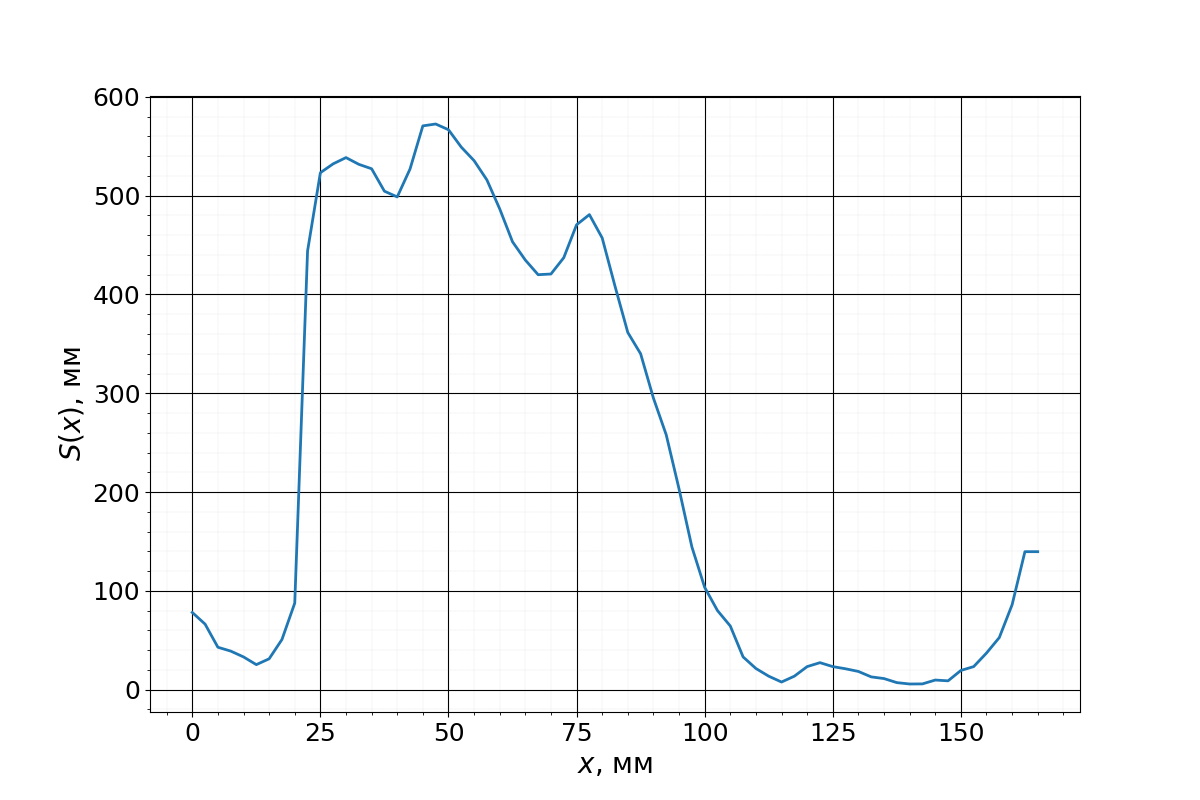
\includegraphics[width=0.95\linewidth]{Pictures/VoicePlot.png}
			\caption{Графическое представление $S(x)$}
		\end{figure}
	
		Найдем первые 4 собственных значения и соответствующие собственные функции для этого уравнения. 
		
		Обращаясь к методу стрельбы, распишем получившиеся системы. Пусть $u = \Psi$, $v = \Psi'_x$, $A = \frac{\partial u}{\partial \lambda}$, $B = \frac{\partial v}{\partial \lambda}$, а дополнительное условие:
		\begin{equation*}
			F(\lambda) = 8\sqrt{S(L)}\Psi'_x(L) + 3\pi\sqrt{\pi}\Psi(L) = 8\sqrt{S(L)}v(L) + 3\pi\sqrt{\pi}u(L).
		\end{equation*}
	
		Тогда:
		\begin{equation*}
			\begin{cases}
				u' = v, \\
				v' = -\lambda^2 u - v \frac{S'(x)}{S(x)}, \\
				u(0) = 1, \\
				v(0) = 0.
			\end{cases}
		\end{equation*}
		
		Условие $u(0) = 1$ выбрано потому, что функция $\Psi(x)$ определена с точностью до постоянного множителя (который ищется из условия нормировки).
		
		На $A$ и $B$ будет система:
		\begin{equation*}
			\begin{cases}
				\frac{dA}{dx} = B, \\
				\frac{dB}{dx} = -2\lambda u - \lambda^2 A - B\frac{S'(x)}{S(x)}, \\
				A(0) = 0, \\
				B(0) = 0
			\end{cases}
		\end{equation*}
	
		Тогда также:
		\begin{equation*}
			F'(\lambda) = 8\sqrt{S(L)}\frac{\partial v}{\partial \lambda}(L) + 3\pi\sqrt{\pi}\frac{\partial u}{\partial \lambda}(L) = 8\sqrt{S(L)} B(L) + 3\pi\sqrt{\pi} A(L).
		\end{equation*}
		
		
		\tocsubsection{Результаты}
		Приведем графики первых нескольких собственных состояний.
		
		\begin{itemize}
			\item $\lambda_1 \approx 0.0025707$ мм$^{-1}$
			\begin{figure}[h!]
				\centering
				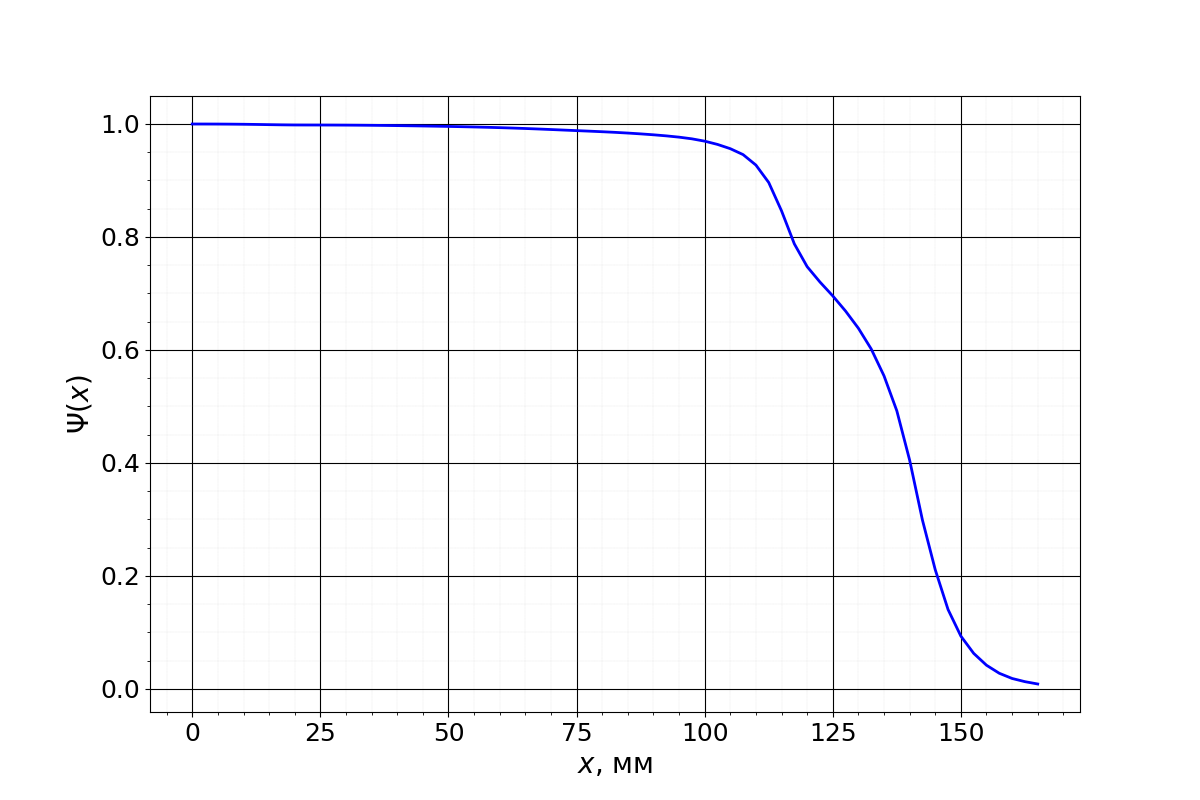
\includegraphics[width=0.92\linewidth]{Pictures/Normal/1.png}
				\caption{График решения при $\lambda = \lambda_1$}
			\end{figure}
		
			\newpage
			\item $\lambda_2 \approx 0.0421654$ мм$^{-1}$
			\begin{figure}[h!]
				\centering
				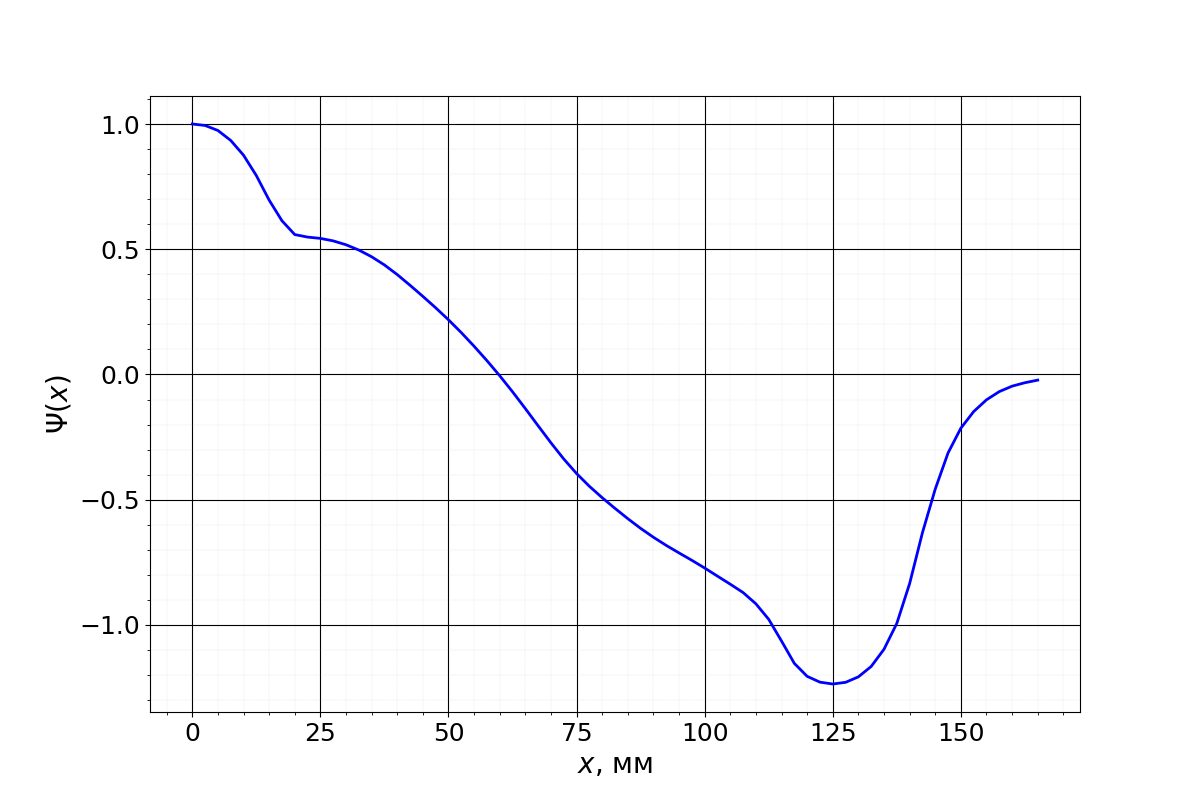
\includegraphics[width=0.92\linewidth]{Pictures/Normal/2.png}
				\caption{График решения при $\lambda = \lambda_2$}
			\end{figure}
		
		
			\item $\lambda_3 \approx 0.0656407$ мм$^{-1}$
			\begin{figure}[h!]
				\centering
				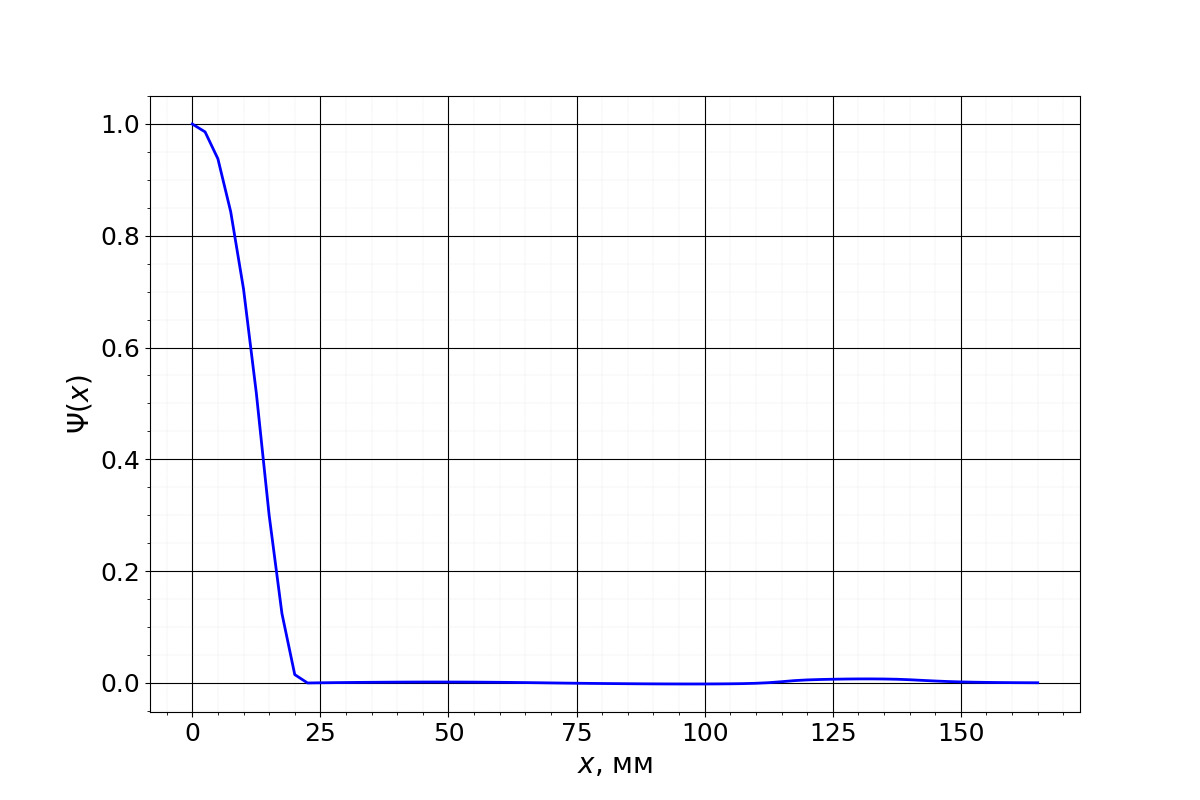
\includegraphics[width=0.92\linewidth]{Pictures/Normal/3.png}
				\caption{График решения при $\lambda = \lambda_3$}
			\end{figure}
		
			\newpage
			\item $\lambda_4 \approx 0.0833594$ мм$^{-1}$
			\begin{figure}[h!]
				\centering
				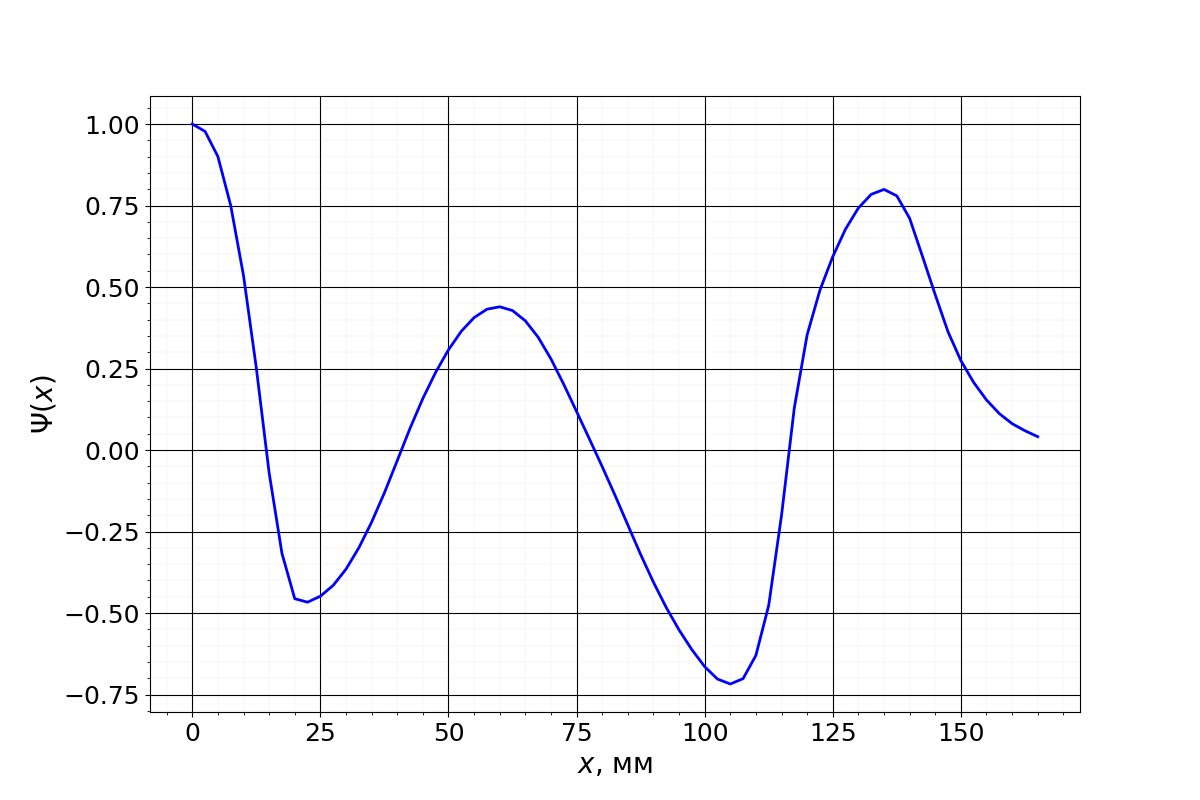
\includegraphics[width=0.92\linewidth]{Pictures/Normal/4.png}
				\caption{График решения при $\lambda = \lambda_4$}
			\end{figure}
		
		
			\item $\lambda_5 \approx 0.1134456$ мм$^{-1}$
			\begin{figure}[h!]
				\centering
				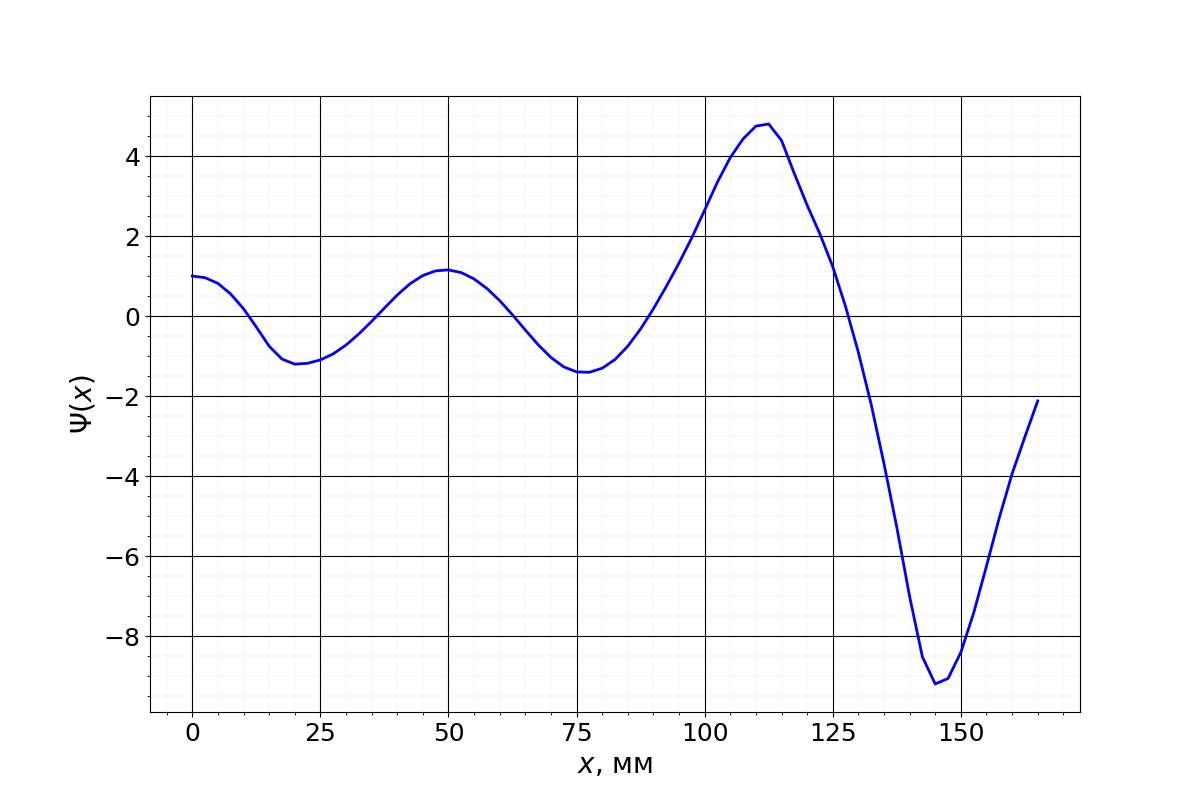
\includegraphics[width=0.92\linewidth]{Pictures/Normal/5.png}
				\caption{График решения при $\lambda = \lambda_5$}
			\end{figure}
		
		
			\newpage
			\item $\lambda_6 \approx 0.1182225$ мм$^{-1}$
			\begin{figure}[h!]
				\centering
				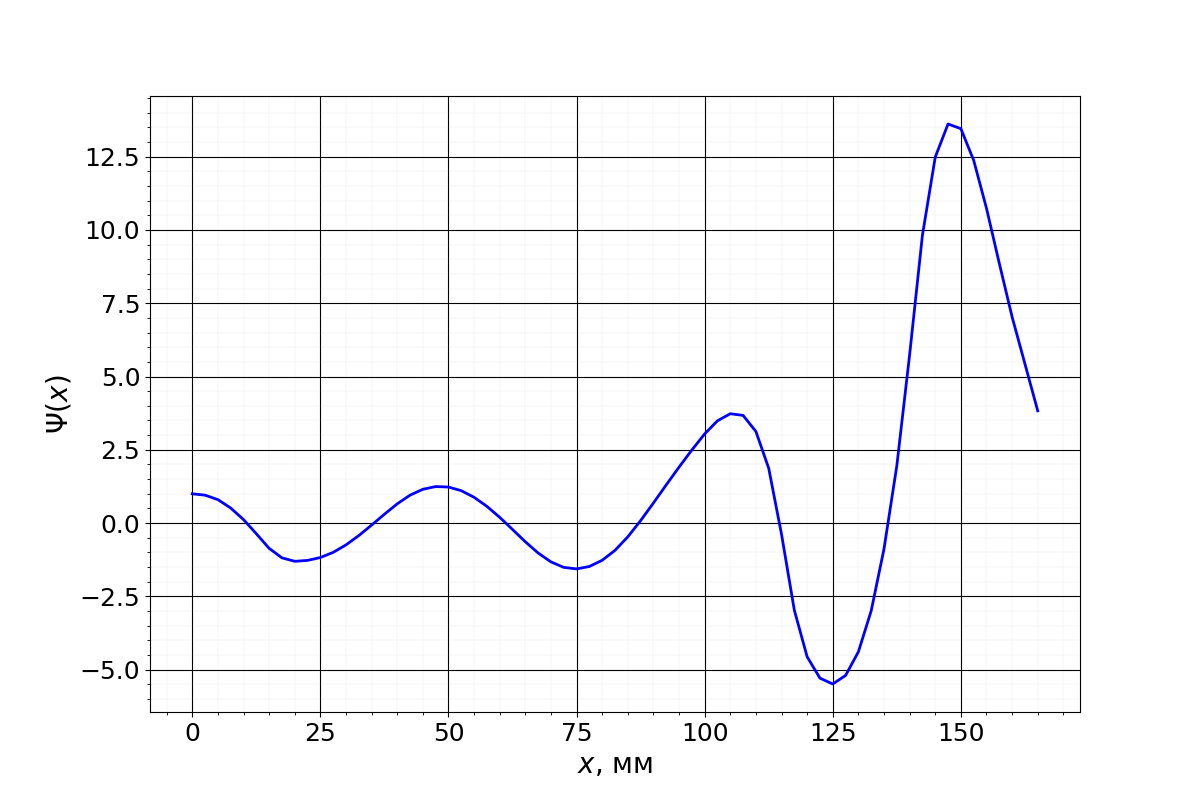
\includegraphics[width=0.92\linewidth]{Pictures/Normal/6.png}
				\caption{График решения при $\lambda = \lambda_6$}
			\end{figure}
		
		
			\item $\lambda_7 \approx 0.1492184$ мм$^{-1}$
			\begin{figure}[h!]
				\centering
				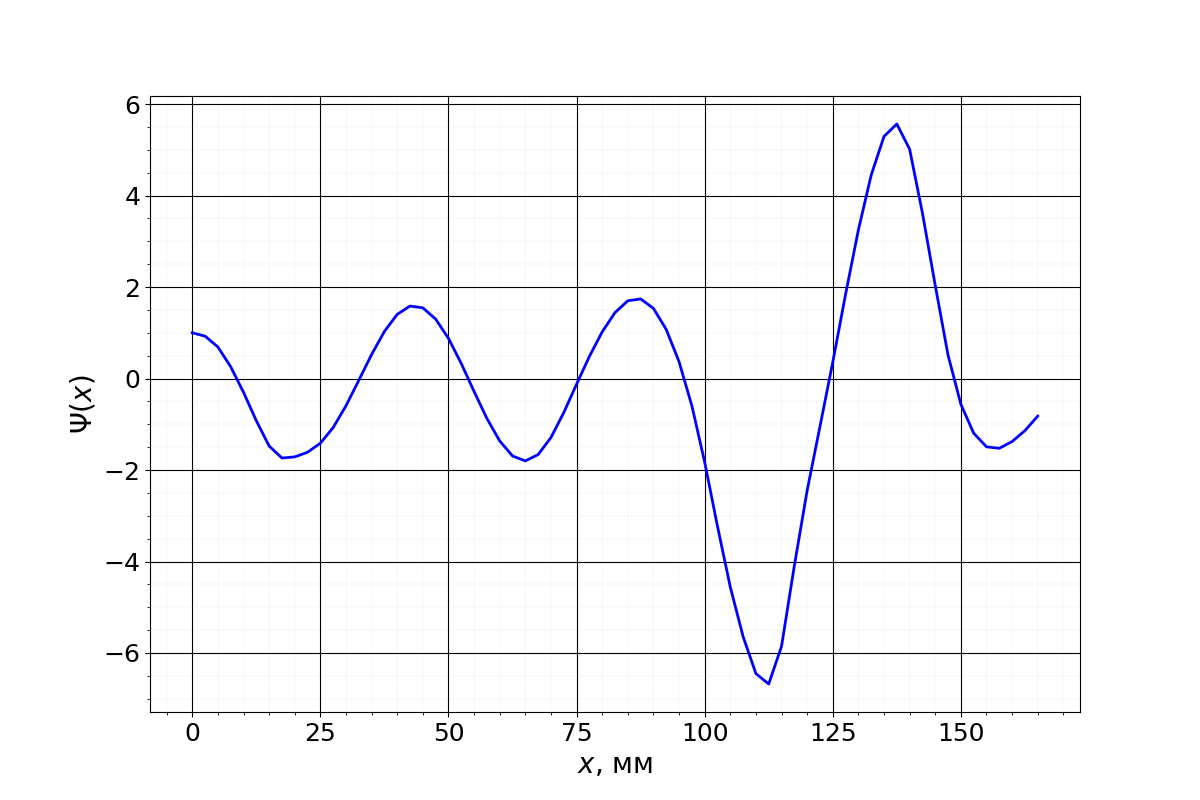
\includegraphics[width=0.92\linewidth]{Pictures/Normal/7.png}
				\caption{График решения при $\lambda = \lambda_7$}
			\end{figure}
		
		
			\newpage
			\item $\lambda_8 \approx 0.1846243$ мм$^{-1}$
			\begin{figure}[h!]
				\centering
				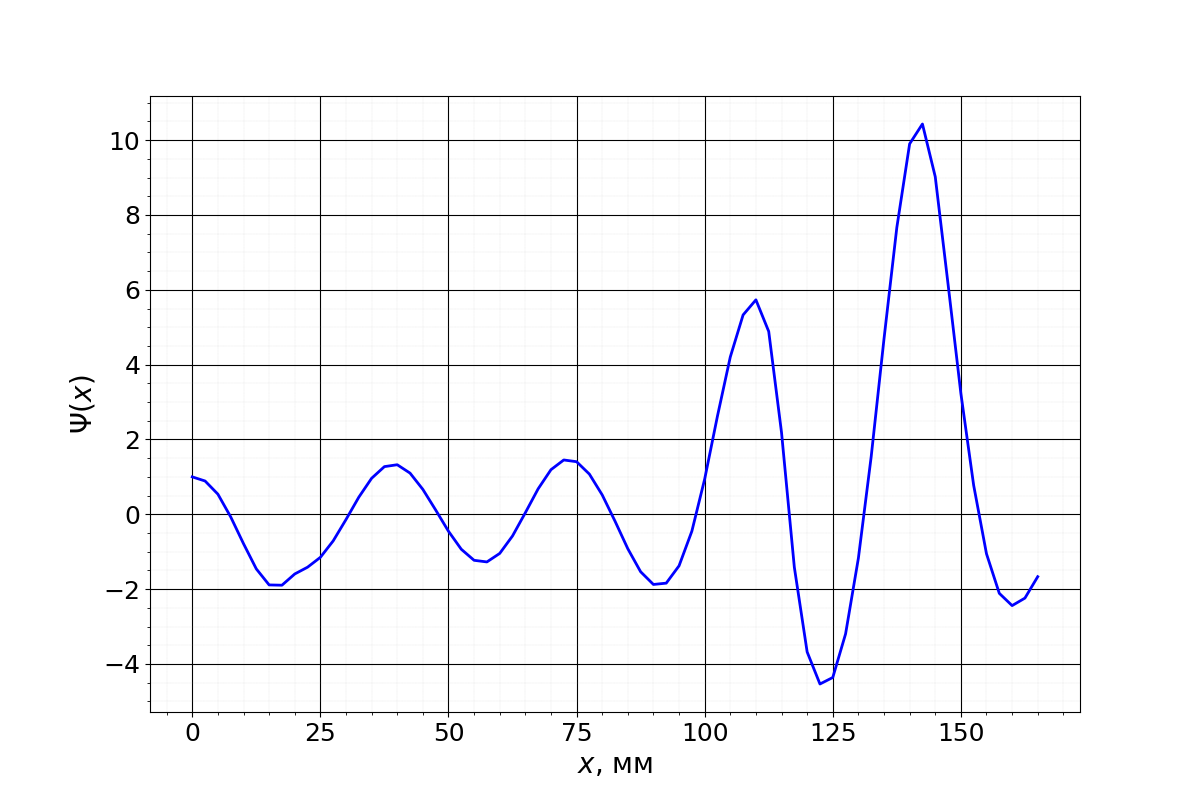
\includegraphics[width=0.92\linewidth]{Pictures/Normal/8.png}
				\caption{График решения при $\lambda = \lambda_8$}
			\end{figure}
		
		\end{itemize}
	
	
		\newpage
		Кажется, что графики выглядят довольно случайно, но это не так. Построим все эти графики в одном фиксированном масштабе.
		
		\begin{figure}[h!]
			\centering
			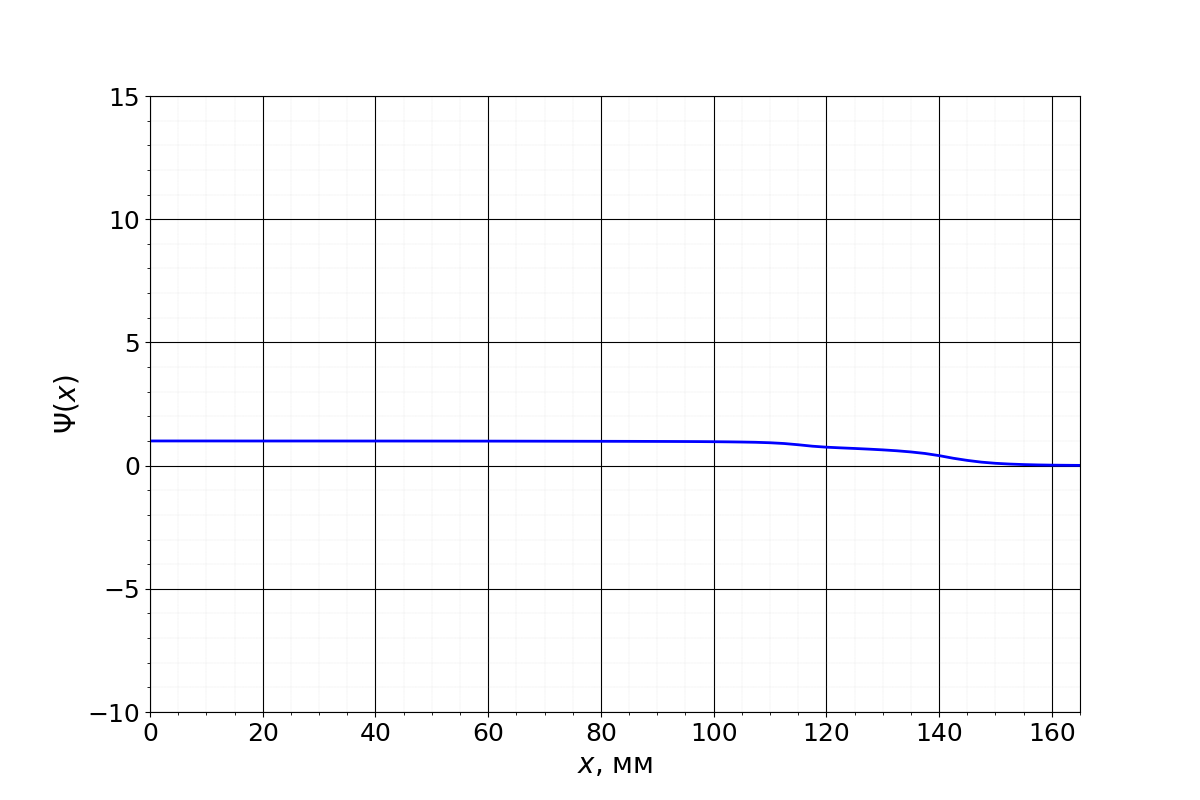
\includegraphics[width=0.92\linewidth]{Pictures/Scaled/1_Scaled.png}
			\caption{График решения при $\lambda = \lambda_1$}
		\end{figure}
		

		\begin{figure}[h!]
			\centering
			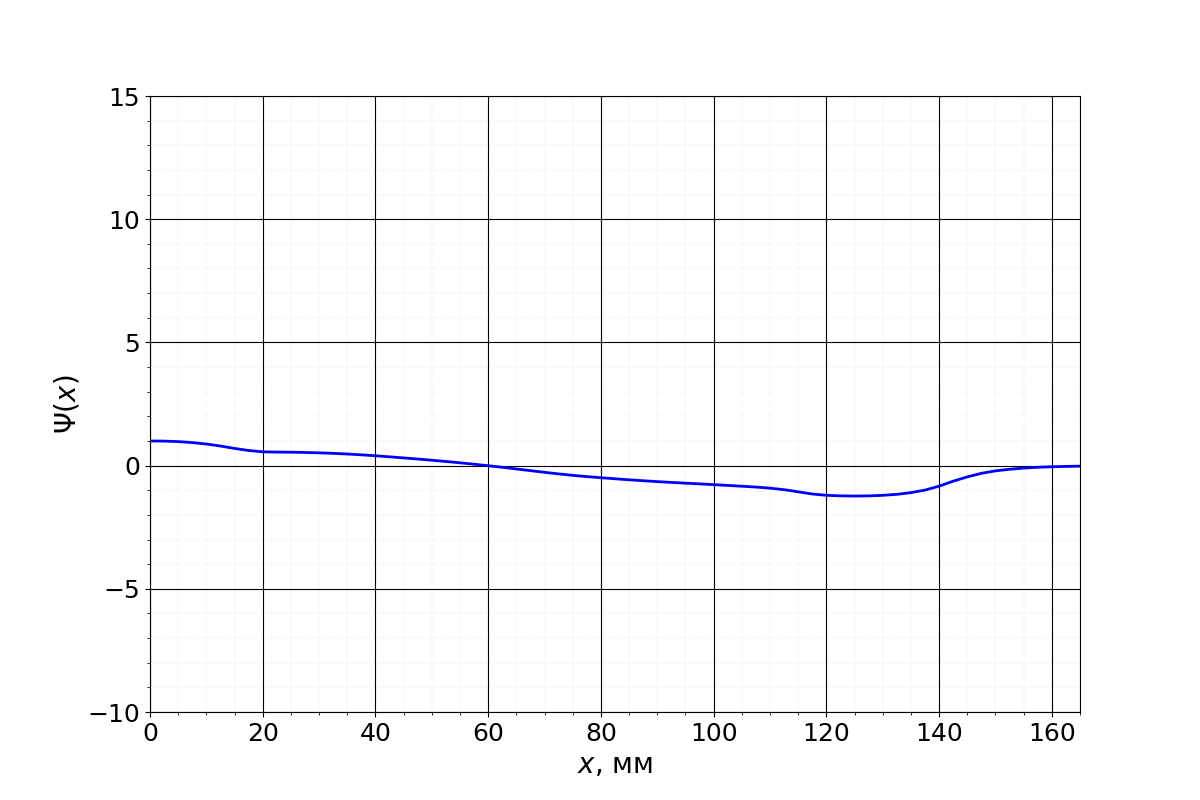
\includegraphics[width=0.92\linewidth]{Pictures/Scaled/2_Scaled.png}
			\caption{График решения при $\lambda = \lambda_2$}
		\end{figure}
		
		
		\newpage			
		\begin{figure}[h!]
			\centering
			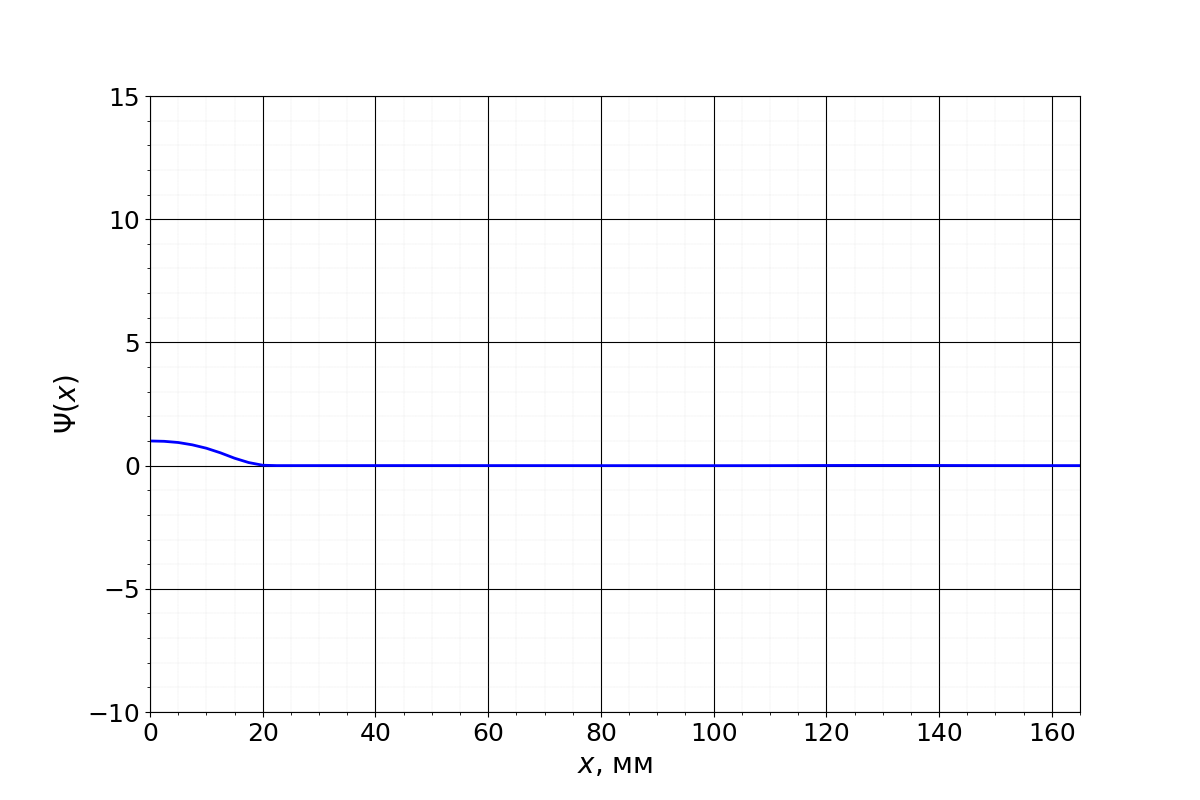
\includegraphics[width=0.92\linewidth]{Pictures/Scaled/3_Scaled.png}
			\caption{График решения при $\lambda = \lambda_3$}
		\end{figure}
		
		
		\begin{figure}[h!]
			\centering
			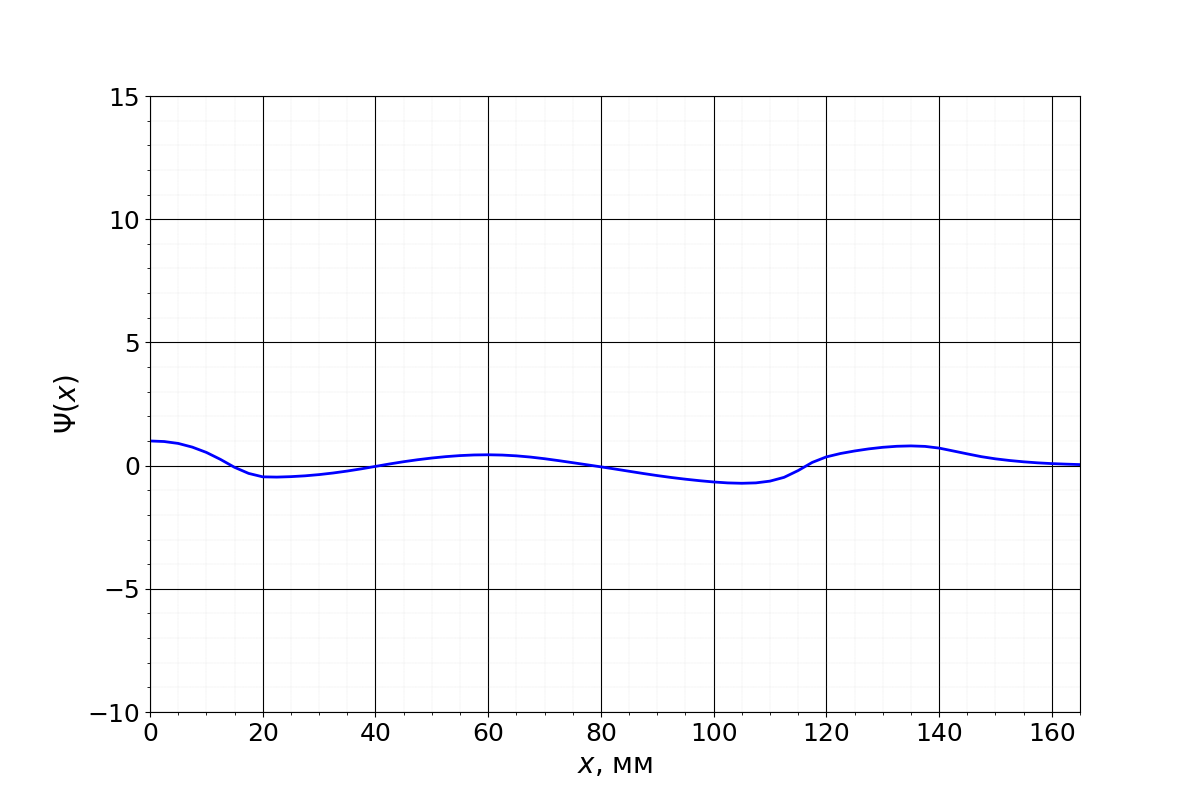
\includegraphics[width=0.92\linewidth]{Pictures/Scaled/4_Scaled.png}
			\caption{График решения при $\lambda = \lambda_4$}
		\end{figure}
		

		\newpage
		\begin{figure}[h!]
			\centering
			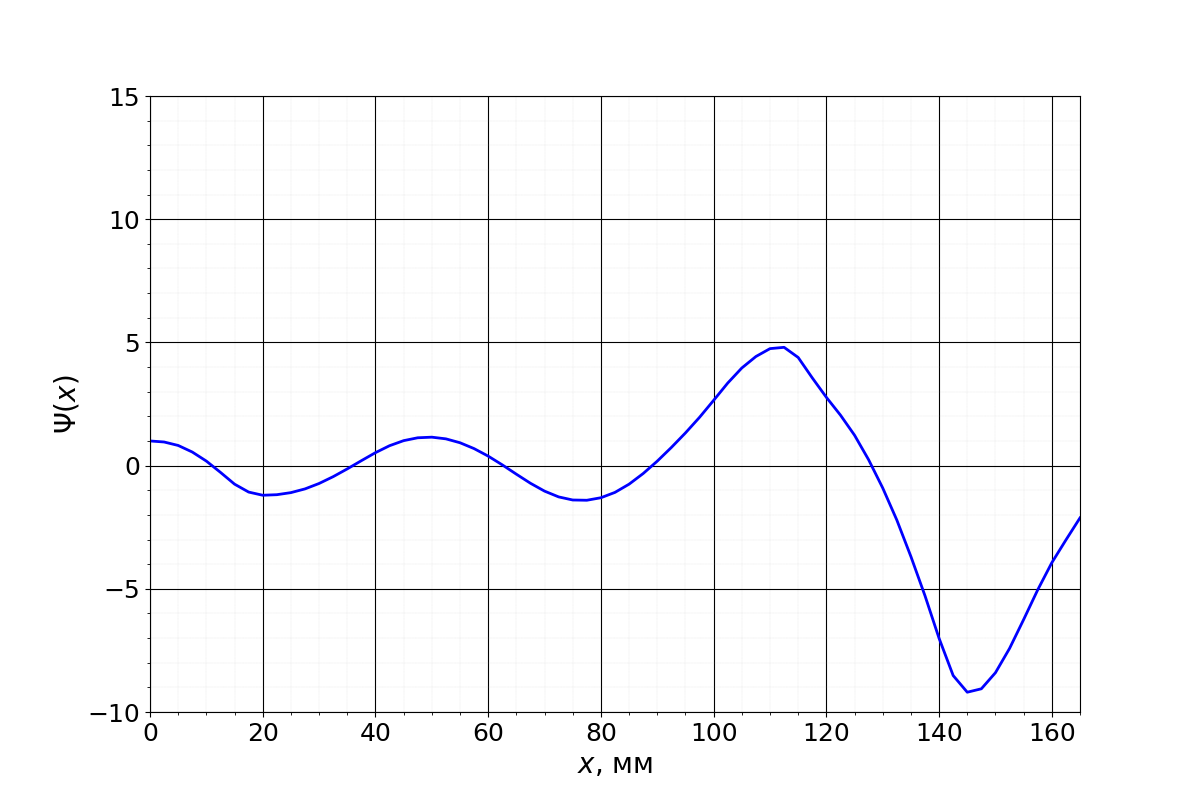
\includegraphics[width=0.92\linewidth]{Pictures/Scaled/5_Scaled.png}
			\caption{График решения при $\lambda = \lambda_5$}
		\end{figure}
		
		
		\begin{figure}[h!]
			\centering
			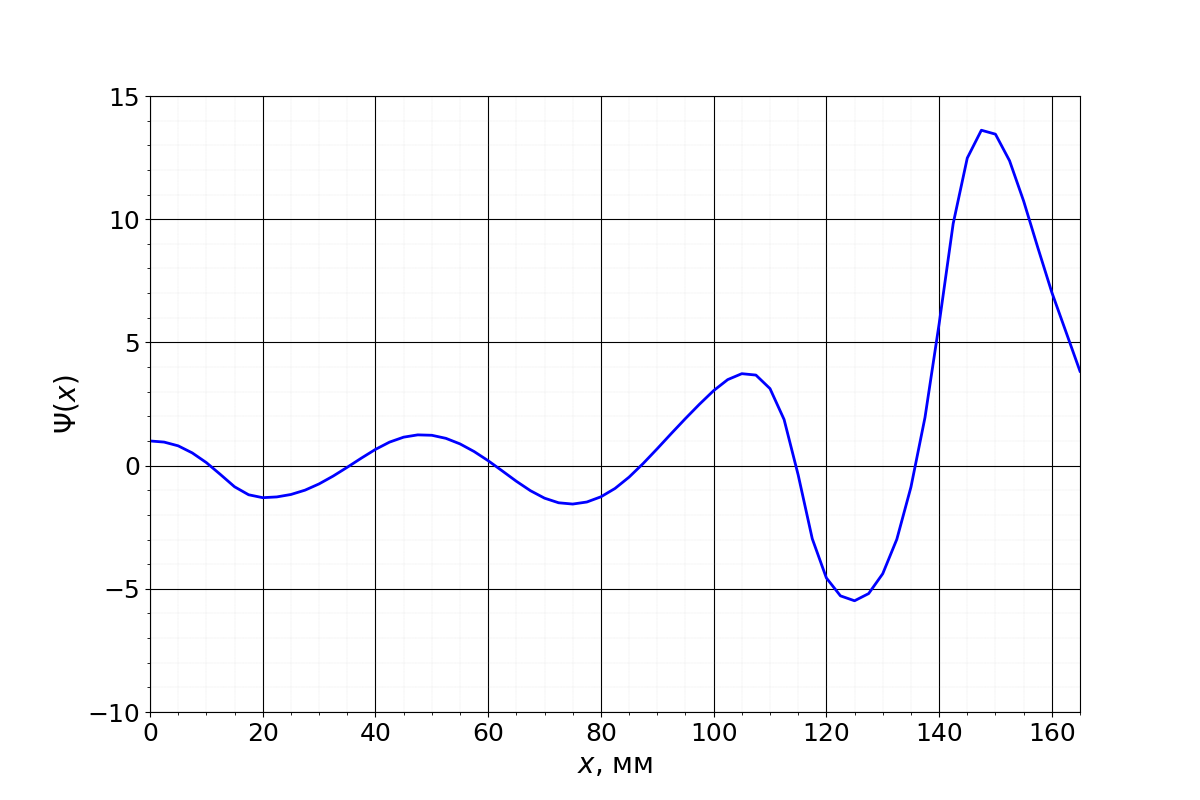
\includegraphics[width=0.92\linewidth]{Pictures/Scaled/6_Scaled.png}
			\caption{График решения при $\lambda = \lambda_6$}
		\end{figure}
		
		
		\newpage			
		\begin{figure}[h!]
			\centering
			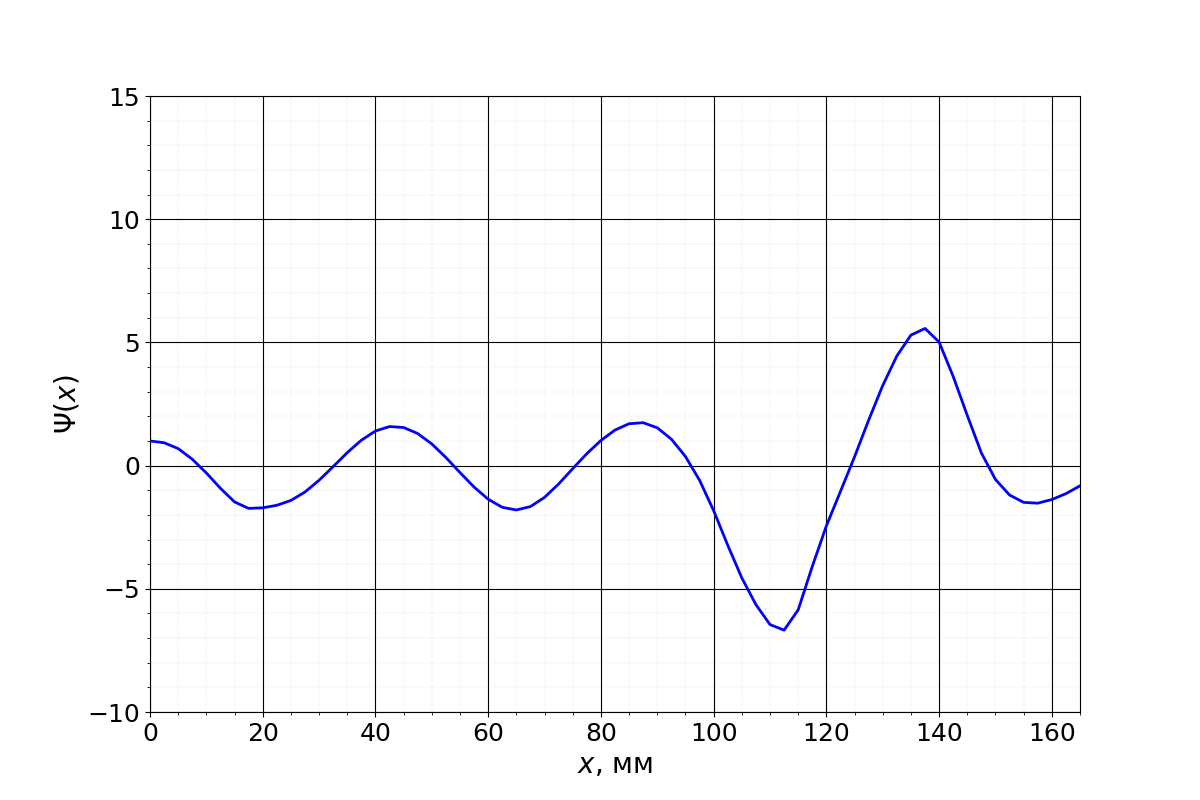
\includegraphics[width=0.92\linewidth]{Pictures/Scaled/7_Scaled.png}
			\caption{График решения при $\lambda = \lambda_7$}
		\end{figure}
		
		

		\begin{figure}[h!]
			\centering
			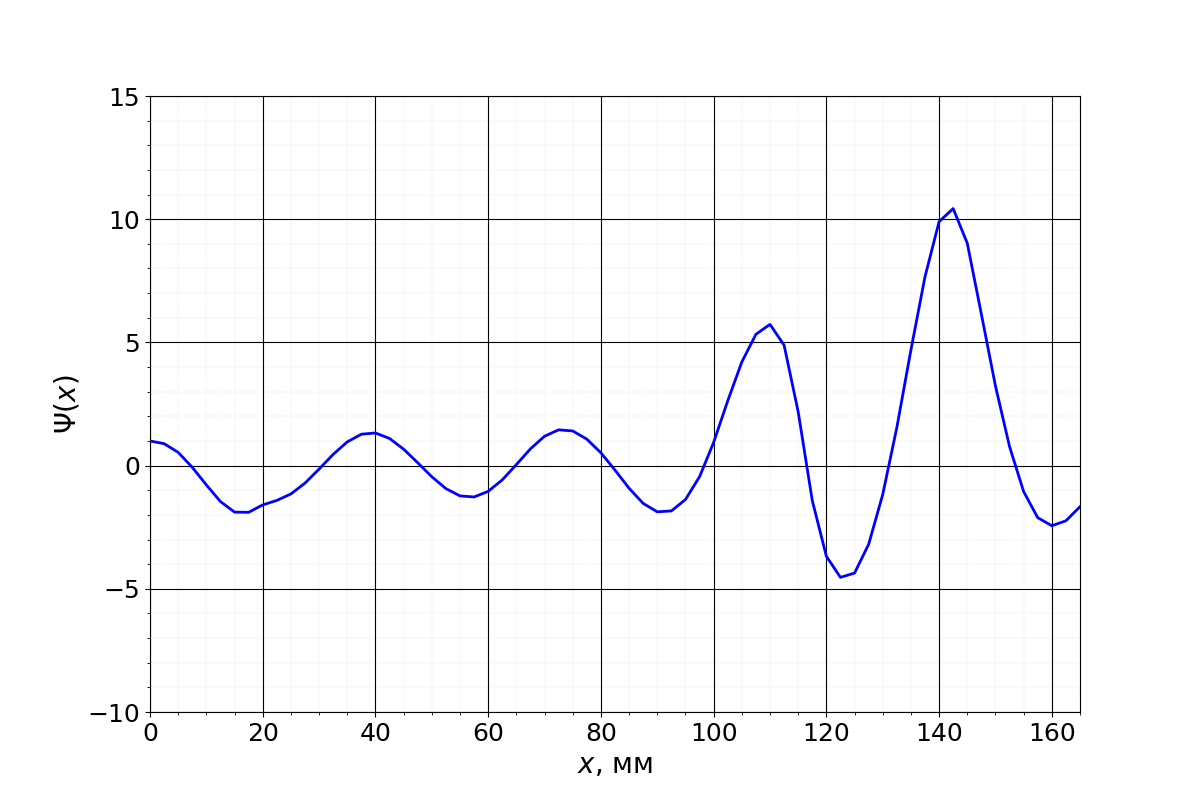
\includegraphics[width=0.92\linewidth]{Pictures/Scaled/8_Scaled.png}
			\caption{График решения при $\lambda = \lambda_8$}
		\end{figure}
		
		Получается своеобразная волна! И она сжимается. Это и понятно, мы рассматриваем резонатор.

		Чтобы лучше увидеть движение этой волны, можно посмотреть Scaled.gif файл.

	
		
		\tocsection{Вывод}
		В работе был использован метод стрельбы для нахождения собственных чисел и состояний уравнения, описывающего голосовой тракт как резонатор.
		
		
\end{document}